\providecommand{\main}{../../..}
\documentclass[\main/dresen_thesis.tex]{subfiles}

\begin{document}
  \subsection{D17}\label{ch:lss:d17}

    \begin{figure}[ht]
      \centering
      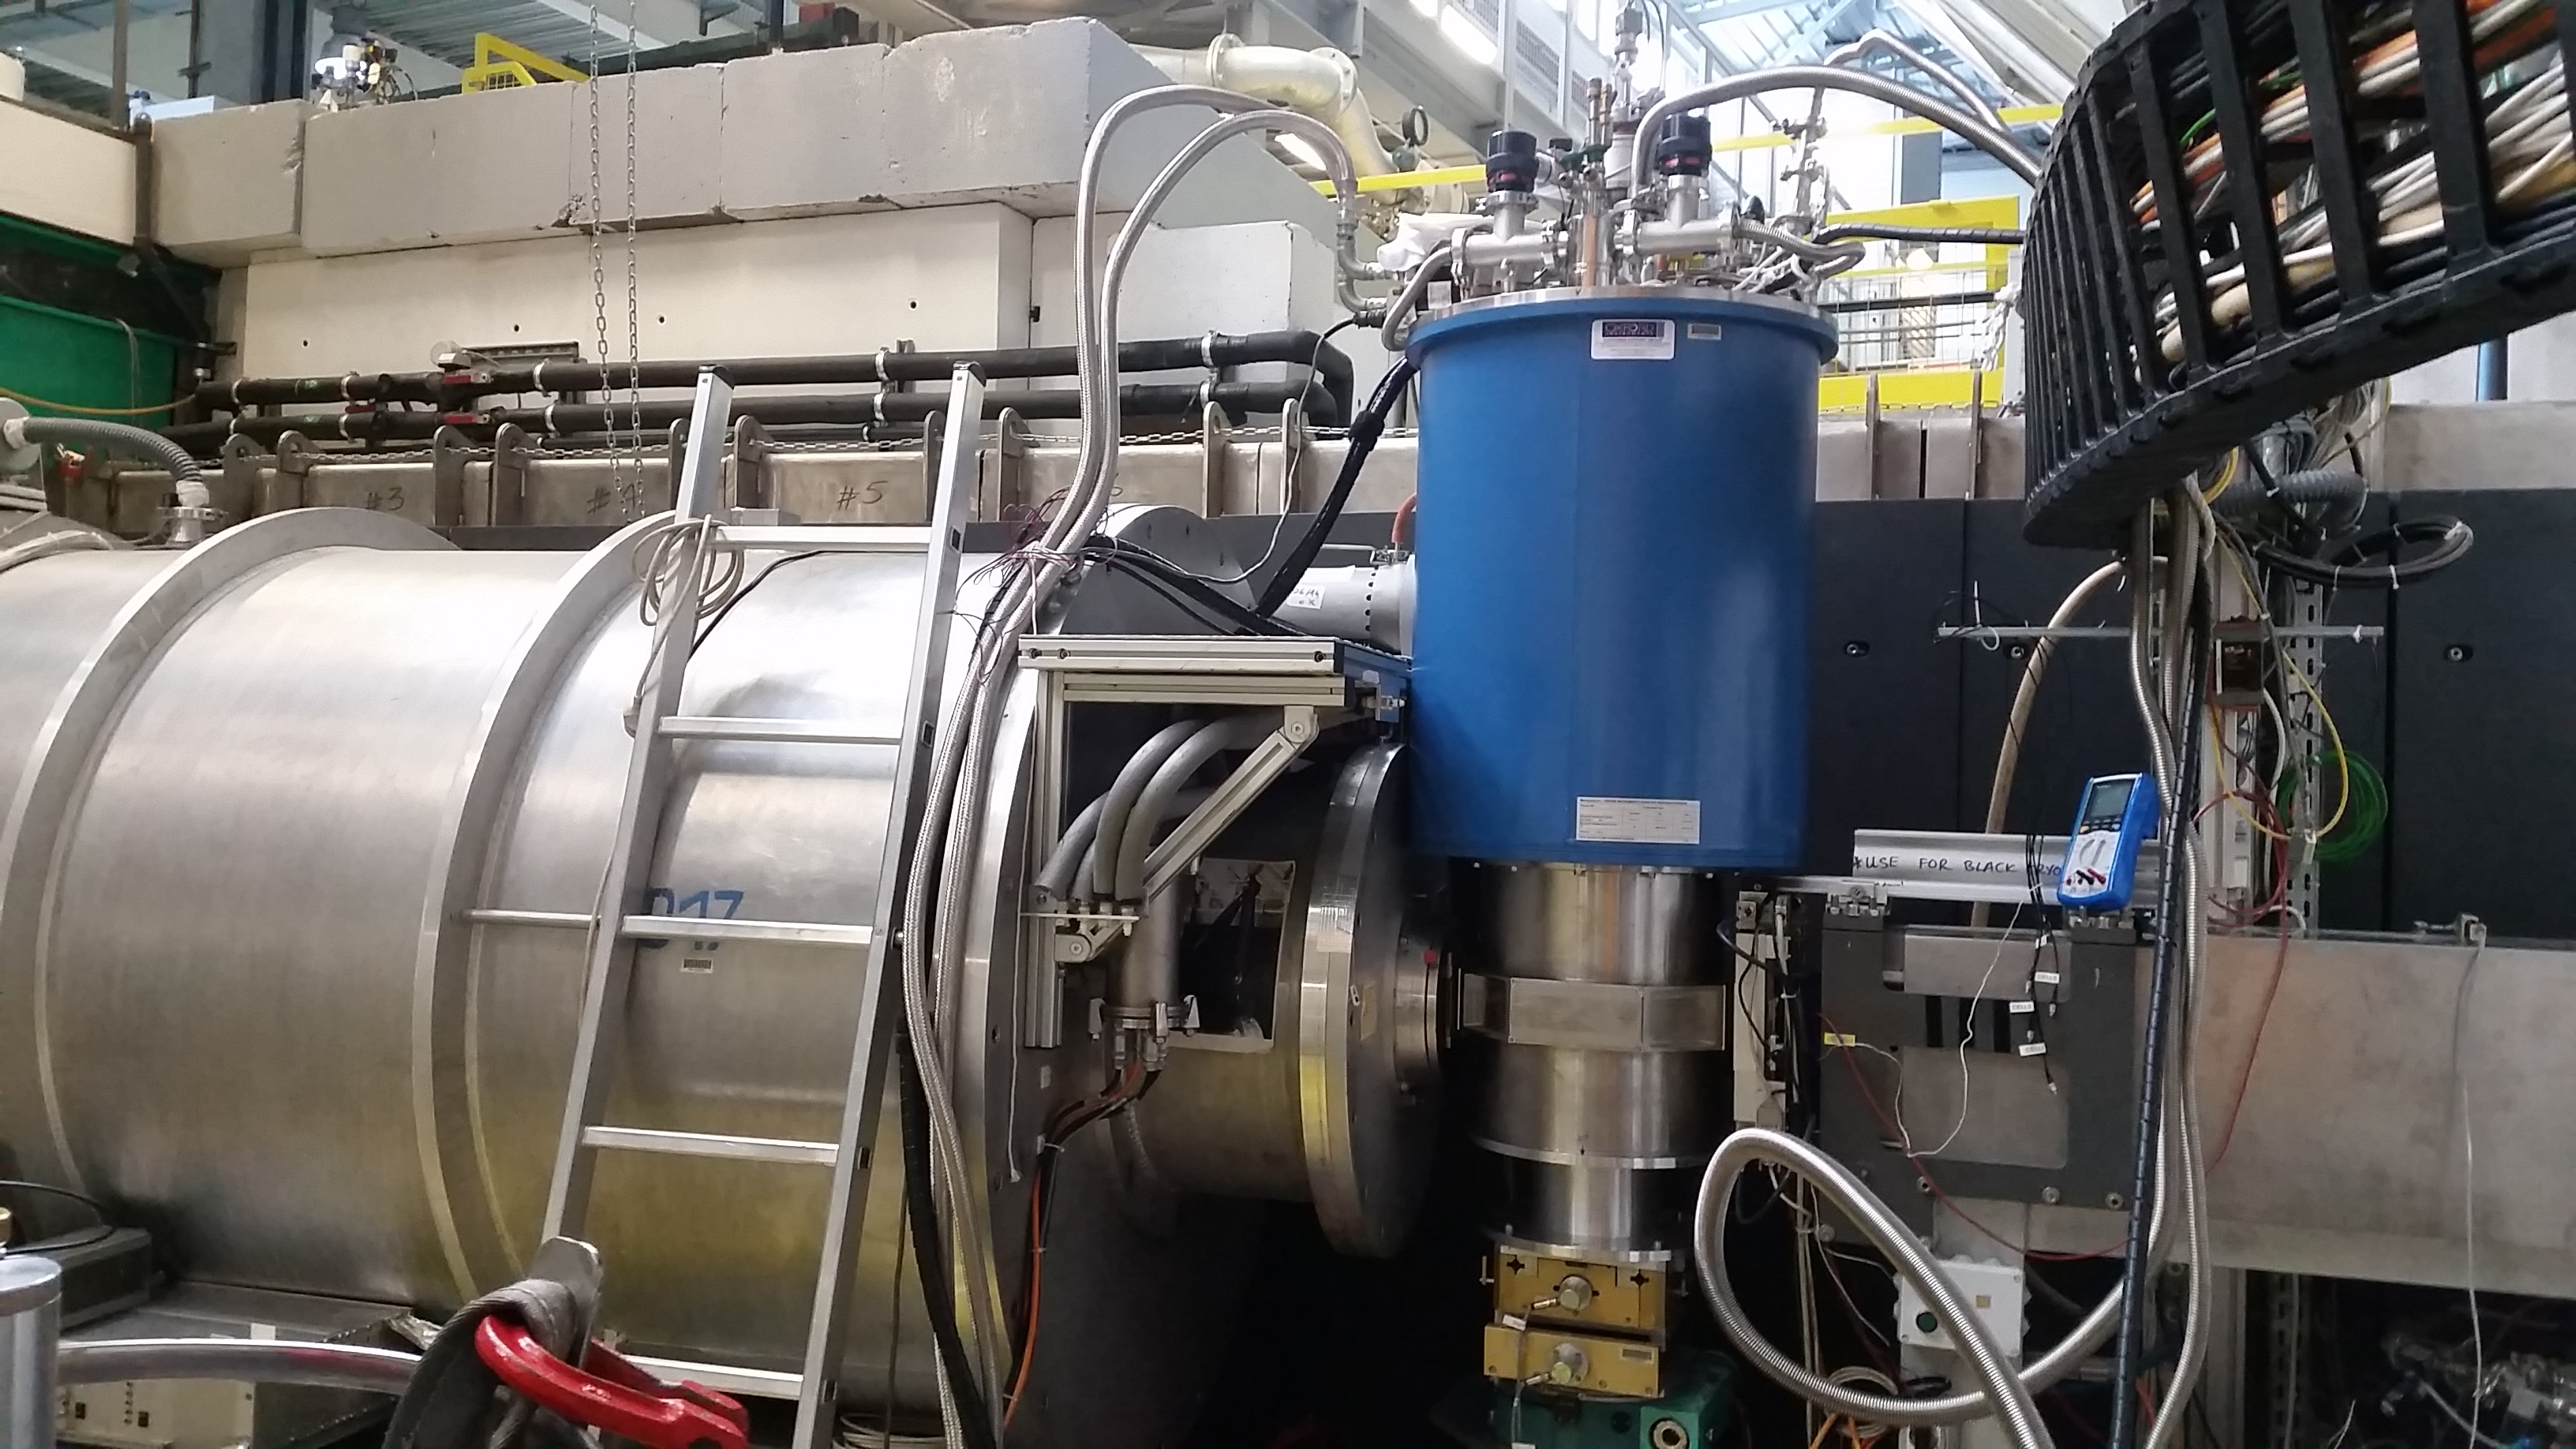
\includegraphics[width=0.49\textwidth]{appendix_instruments_d17}
      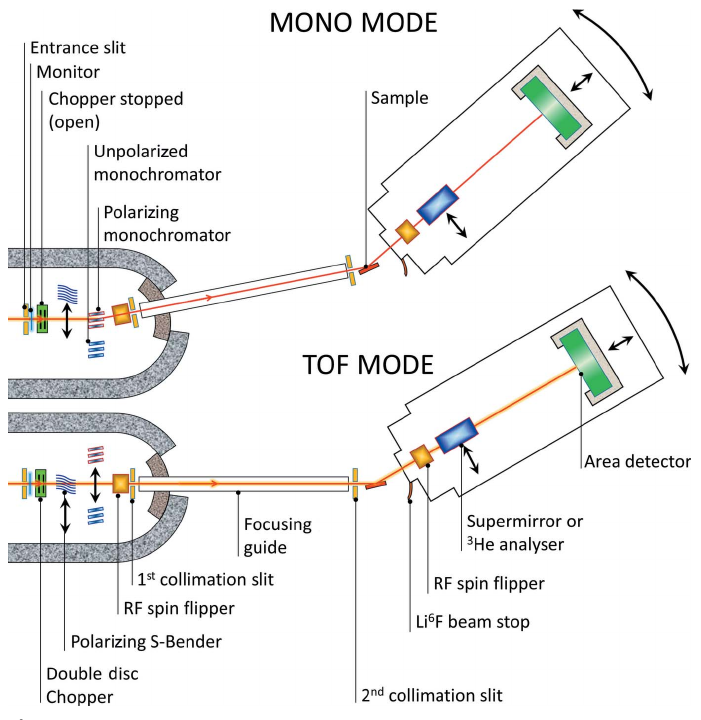
\includegraphics[width=0.49\textwidth]{appendix_instruments_d17Setup}
      \caption{\label{fig:lss:d17}D17 at Institut Laue-Langevin, a time-of-flight instrument used for (polarized) neutron reflectometry (schematics reproduced from \cite{Saerbeck_2018_Recen}).}
    \end{figure}
    The D17 instrument \cite{Saerbeck_2018_Recen} is a polarized neutron reflectometer at the Institute Laue-Langevin, which can be operated in monochromatic and time-of-flight mode (TOF), where the latter is used in this thesis.
    In the TOF mode, the white neutron beam is collimated over a distance of $L_\mathrm{CSD} \eq 3.4 \unit{m}$ and the detector can be moved for a sample-to-detector distance of $L_\mathrm{SSD} \eq 1 \ldots 3.1 \unit{m}$.
    The detector has a spatial resolution of $2.2 \times 5.2 \unit{mm}$ (FWHM) with an active area of $473 \times 250 \unit{mm^2}$.

    The polarisation of neutrons in a wavelength of $4 \ldots 20 \unit{\angstrom}$ is achieved by an \ch{Fe}/\ch{Si} polarising multilayer S-bender, which has a polarization efficiency of over $99 \unit{\%}$ for the whole wavelength band.
    The RF flipper has a flipping efficiency close to $99 \unit{\%}$ for wavelengths $\lambda < 10 \unit{\angstrom}$ and linearly decreases to $>96 \%$ for the higher wavelength.

    For data reduction, the COSMOS software \cite{Gutfreund_2018_Towar} is used, which implements the correction for polarization efficiencies, estimates the resolution and allows to scale overlapping data sets measured at multiple incident angles on one another.
\end{document}